\documentclass[11pt]{report}
\usepackage{blindtext}
\usepackage[margin=1in]{geometry}
\usepackage{graphicx}
\usepackage{verbatim}
\title{Thanks Corporation Database Project\\CMSI 486 Enterprise Project --- Fall 2014}
\author{Edward Bramanti}

\providecommand\phantomsection{}


\renewcommand\thechapter{\Roman{chapter}}
\renewcommand\thesection{\thechapter.\arabic{section}}

\usepackage{tocloft}
\setlength{\cftchapnumwidth}{3em}
\setlength{\cftsecnumwidth}{3.5em}
\setlength{\cftsubsecnumwidth}{4em}

\begin{document}
\clearpage
\phantomsection
\addcontentsline{toc}{chapter}{
    \protect\numberline{I}Title Page}
\maketitle
\clearpage
\phantomsection
\addcontentsline{toc}{chapter}{
    \protect\numberline{II}Table of Contents}
\tableofcontents
\setcounter{page}{2}
\setcounter{chapter}{2}
\chapter{Description of the Enterprise}

Thanks is an effective, entirely digital, multi-purpose employee recognition system. The database will consist of many different companies who will pay for a service that makes recognizing employees simple and meaningful. This will allow the Thanks database to be used in a way that is unique to each company using the service.

The enterprise in question will make it much easier for employees to recognize one another across their company. As companies grow, it becomes difficult to maintain an atmosphere of employee worth. This growing size represents a problem as individual employees can feel like their work goes unnoticed in their company. “Thanks” provides a remedy for that by providing a digital way to send recognition to any employee quickly.

In an organization, there will be one user type with some special attributes. For example, an executive will be a special user type and will be denoted with special attributes. When opening the thanks form, it will be necessary to present a list of all employees in the company. A list of employees would appear with these attributes: name, position and department. This would provide employees with a clear snapshot on everyone’s role in the company if they saw a fellow employee do something amazing and was not sure what position they occupied in the company. Users will be able to send other users the primary data type known as Thanks. For each thank, we have a user that gives the Thanks and a user that receives the Thanks. This demonstrates the personal aspect of recognition, as an employee recognizes a specific employee directly.

A Thanks also contains an area for an employee to write a message so they can explain what they are thanking the employee for. This allows for personalization of the Thanks so that employees can be detailed on the outstanding work their coworkers are doing. Finally, companies will be able to define a custom attribute for the last part of the Thanks, which will be represented as values the company wants to promote. The advantage of this value is that companies, depending on their mission statements and core beliefs, will be able to tailor this field to encourage specific attributes that represent the company within employees.

Thanks represents a social network within a company than it is a private thanking system. Messages will display on a live feed all of the “Thanks” being given around the company. Employees will be able to easily see the interaction and encouragement being spread amongst their acquaintances. The potential of “Thanks” is enormous, which is why a specific structure around a public space of thanks combined with personalized instances and explanations of employee worth are necessary in this database design.\\

\clearpage
Here are a set of questions employees, department heads or executives may pose when retrieving data:
\begin{enumerate}
    \item List all employees in the company ``I Love Thanks".
    \item Which department has received the most Thanks in the company?
    \item Return a list of all employees who have nicknames.
    \item List all company values for the ``I Love Thanks" company.
    \item Which department head has received the most Thanks in the company?
    \item Which one of Julia Crow's Thanks she gave received the most likes?
    \item Who has never received a Thanks within a company?
    \item Who is the newest employee to have joined the company?
    \item How many Thanks were posted in the company on October 20, 2014?
    \item List the executives in the company ``I Love Thanks".
\end{enumerate}

\chapter{Definition of Environment}

\section{Input and Report Forms}
\section{Assumptions}
\section{User-Oriented Data Dictionary}
\section{Cross-Reference Table}

\chapter{Enterprise Database Design}

\section{Logical Model of the Enterprise}
\subsection{List of Entities and Attributes}

\begin{itemize}
\item Employee
    \begin{itemize}
    \item eid: Employee ID
    \item name: Employee Name
    \item job\_title: Employee Job Title
    \item photo: Employee Photo
    \item nickname: Employee Nickname
    \item started: Date the Employee Started
    \end{itemize}
\item Department Head - inherits Employee
    \begin{itemize}
    \item headid: Department Head ID
    \end{itemize}
\item Executive - inherits Employee
    \begin{itemize}
    \item execid: Executive ID
    \end{itemize}
\item Department
    \begin{itemize}
    \item did: Department ID
    \item depTitle: Department Title
    \item depDescription: Department Description
    \end{itemize}
\item Company
    \begin{itemize}
    \item cid: Company ID
    \item cTitle: Company Title
    \item founded\_date: Date Company was Founded
    \end{itemize}
\item Thanks
    \begin{itemize}
    \item tid: Thanks ID
    \item thanksdate: Date Thanks was Given
    \end{itemize}
\item Like
    \begin{itemize}
    \item likedate: Date Like was Given
    \end{itemize}
\item Comment
    \begin{itemize}
    \item commentdate: Date Comment was Given
    \end{itemize}
\item Message
    \begin{itemize}
    \item mid: Message ID
    \item message\_text: Text of Message
    \end{itemize}
\item Company Value
    \begin{itemize}
    \item vid: Company Value ID
    \item value\_type: type of company value
    \end{itemize}
\end{itemize}
\clearpage

\subsection{List of Relationships and Attributes}
\begin{itemize}
\item Relationship
\end{itemize}
\clearpage

\subsection{Entity-Relationship Diagram of the Enterprise}

\begin{figure}[!htb]
\centering
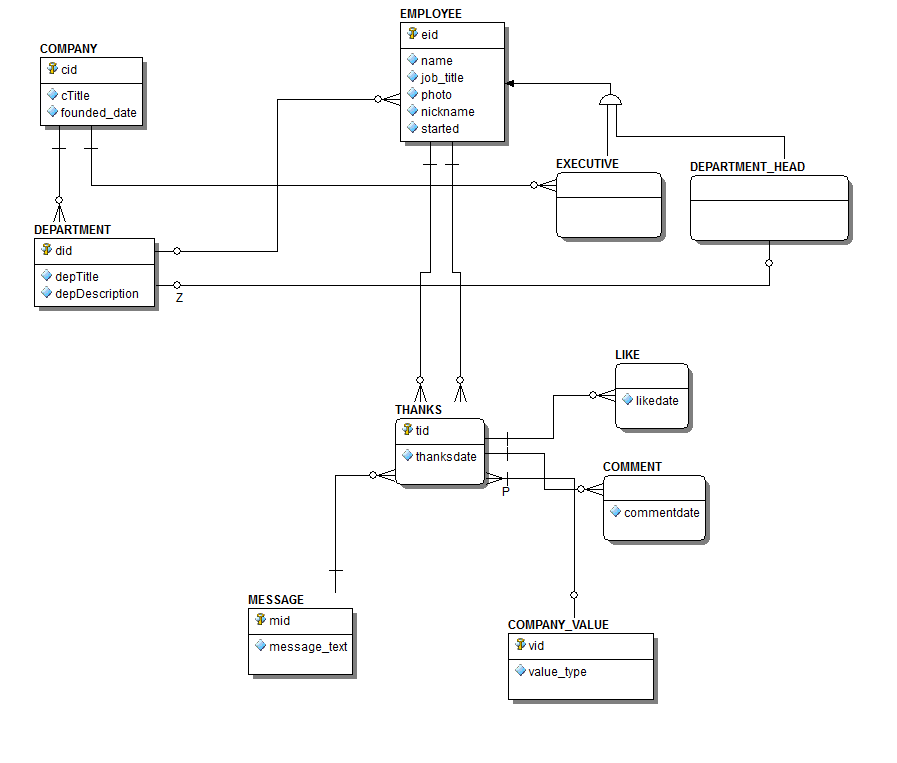
\includegraphics[scale=.7]{./images/ERD11-4.png}
\end{figure}
\clearpage

\section{Conceptual model of the enterprise}
employee(\underline{eid}, name, job\_title, photo, nickname, started) \\

    CK - eid, name, photo

departmenthead(\underline{headid}) \\

executive(\underline{execid}) \\

department(\underline{did}, depTitle, depDescription) \\

    CK - did, depTitle

company(\underline{cid}, cTitle, founded\_date) \\

    CK - cid, cTitle

thanks(\underline{tid}, thanksdate) \\

    CK - tid

like(\underline{tid}, likedate) \\

    CK - tid
    FK - tid REFERENCES thanks.tid

comment(\underline{tid}, commentdate) \\

    CK - tid
    FK - tid REFERENCES thanks.tid

message(\underline{mid}, message\_text) \\

    CK - mid

company\_value(\underline{vid}, value\_type) \\

    CK - vid
\clearpage
\section{Table dictionary}
\section{Attribute dictionary}

\chapter{Database and Query Definition}

\section{Database Definition}
\verbatiminput{sql/ThanksCorporation.sql}
\section{Database Queries}
Given below are 10 example English queries, with their SQL DML used to retrieve the necessary data.
\begin{enumerate}
    \item Bla
\end{enumerate}
\clearpage
\section{Design Tradeoffs and Limitations}

One design tradeoff in its current state is the lack of Thanks being tied to the company. In order to gain access to all thanks by company, multiple joins must be performed instead of having a relationship directly between company and the thanks given within a company. This may be remedied in the future by adding a relationship between THANKS and COMPANY.\\

Another design tradeoff is the lack of relationship between COMPANY and COMPANY\_VALUE. This issue is very similar to the tradeoff listed above: multiple joins are required in order to get the COMPANY\_VALUE when a relationship could be tied between COMPANY and COMPANY\_VALUE.\\

Finally, one design difficulty was in how employees are linked to thanks. Two foreign keys are required in a Thanks entity, which have been aliased to `to' and `from'. Both of these reference an employee, and can create difficulty due to the aliasing of the foreign keys. However, this is necessary in the current implementation.

\end{document}
